% -*-coding: utf-8 -*-
% Держать в начале каждого файла!

\documentclass[a4paper, 12pt]{extarticle}
\usepackage{metod}

\MTDSetPhysSection{Механика}
\MTDSetTitle{Определение модуля Юнга}
\MTDDesignator{М--9B}
\MTDSetGrade{10}

\MTDSetAuthors{И.~Н.~Грачева, В.~И.~Гребенкин, А.~Е.~Иванов, И.~А.~Коротова,
Е.~И.~Красавина, А.~В.~Кравцов, Н.~С.~Кулеба, Б.~В.~Падалкин,
Г.~Ю.~Шевцова, Т.~С.~Цвецинская}

\MTDSetEditorsGenCase{И.~Н.~Грачевой, А.~Е.~Иванова, А.~В.~Кравцова}

\newcommand{\eps}{\epsilon}

\begin{document}

\MTDTitlePage
\MTDInfoPage

\setcounter{section}{9}

\subsection{Цель работы}
Экспериментальное определение модуля Юнга в образце и оценка точности метода. 

\subsection{Основные теоретические сведения}
Модуль Юнга "--- характеристика упругих свойств материала, из которого изготовлен образец, не зависящая от размеров и формы образца. В 1676~году Роберт Гук сделал открытие: при растяжении пружины возрастающей силой удлинение пружины растет прямо пропорционально этой силе. Закон выполняется и тогда, когда удлинение пружины в несколько раз превосходит ее первоначальную длину. По закону Гука происходят деформации во многих случаях растяжения и сжатия, скручивания и изгиба. Например, при растяжении проволоки ее удлинение пропорционально приложенной силе. При растяжении или сжатии стержня сохраняется то же соотношение между изменением длины стержня и приложенной силой. При кручении стержня угол закручивания пропорционален закручивающему моменту силы. Прогиб балки под нагрузкой пропорционален величине нагрузки. Сжатие твердого тела или жидкости дает изменение объема, пропорциональное приложенному давлению. Все свидетельствует о том, что деформация пропорциональна приложенной силе. Однако пределы, в которых могут наблюдаться упругие деформации, у разных материалов и тел различны. Нарушение закона Гука под нагрузкой свидетельствует о близости разрушения образца. Таким образом, задача определения упругих характеристик образца является актуальной при строительстве различных инженерных сооружений.

Кроме формы записи $F = - kx$, где $k$ "--- коэффициент упругости, или жесткость, закон Гука может иметь вид $\sigma = E \eps$, где $\eps$ "--- относительное удлинение образца, а $\sigma$ "--- напряжение, созданное упругой силой. Напряжение измеряется в Паскалях, то есть $\sigma = F/S$, где $S$ "--- площадь поперечного сечения образца. Если образцы из одного и того же материала, но разных диаметров, испытывают одинаковое напряжение, имея одинаковую начальную длину, удлинение у них также будет одинаковым. То есть, отношение напряжения к относительной деформации является постоянной величиной, характеризующей жесткость данного материала. Эта величина называется модулем Юнга и обозначается $E$. Физический смысл модуля Юнга следующий: это такое напряжение, при котором длина образца  увеличится вдвое. Разумеется, это не означает, что такое возможно для любого материала. Тем не менее, численное значение модуля Юнга именно по этой причине так велико для большинства твердых материалов. Если стальная пружина может увеличить свою длину, не разрушаясь, в~5 или 10~раз, то для стальной проволоки это невыполнимо. Прочность проволоки зависит от межатомных сил, которые действуют внутри кристаллической структуры стали. В этих масштабах закон Гука выполняется на расстояниях, сравнимых с межатомными. Этим объясняется тот факт, что длина металлического стержня под нагрузкой в пределах выполнимости закона Гука изменяется не более, чем на~0,05\%.

Ниже приведен график зависимости силы межмолекулярного взаимодействия от расстояния между центрами двух молекул. Часть графика над горизонтальной осью соответствует силе отталкивания, под ней "--- притяжения. Точка пересечения графика с осью расстояний дает положение равновесия, равное удвоенному радиусу молекулы. Если молекулу представить более или менее жестким шариком, то это положение соответствует касанию двух соседних шариков. При сближении их центров на меньшие расстояния, как и на большие, возникают силы, характеризующиеся жирной линией, в небольших пределах около положения равновесия. Эта линия совпадает с прямой, т.~е. сила на малом участке отвечает закону Гука. %"Ниже приведен график"! опасно, лучше сделать ссылку

\begin{figure}[h]
\begin{center}
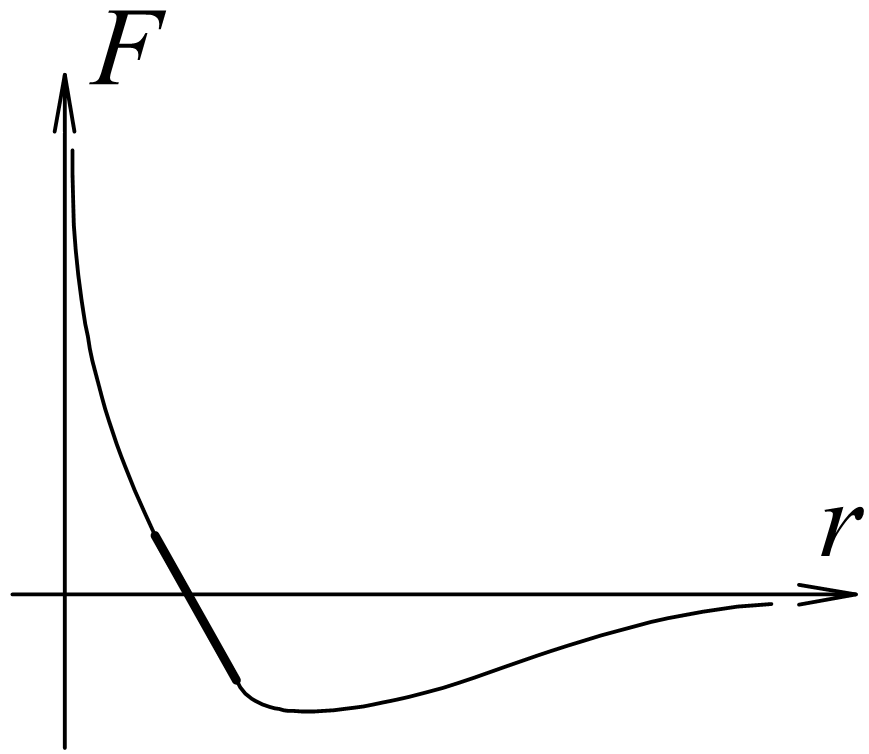
\includegraphics[width=0.4\linewidth, keepaspectratio=true]{M9-IntermolecularForcePlot}
\end{center}
\caption{\label{fig:m9b-plot}}
\end{figure}

Существует несколько разных способов определения модуля Юнга. В этой работе вы познакомитесь с двумя из них: измерение удлинения пружины под действием веса грузов, прикрепленных к ее свободному концу, и измерение прогиба металлической пластины под действием веса грузов, приложенного к ее середине. Для оценки эффективности этих способов, произведя измерения и вычислив модуля Юнга, необходимо определить относительную погрешность результатов. %модулЯ? 

\subsection{Порядок выполнения работы}

\begin{figure}[h]
\begin{center}
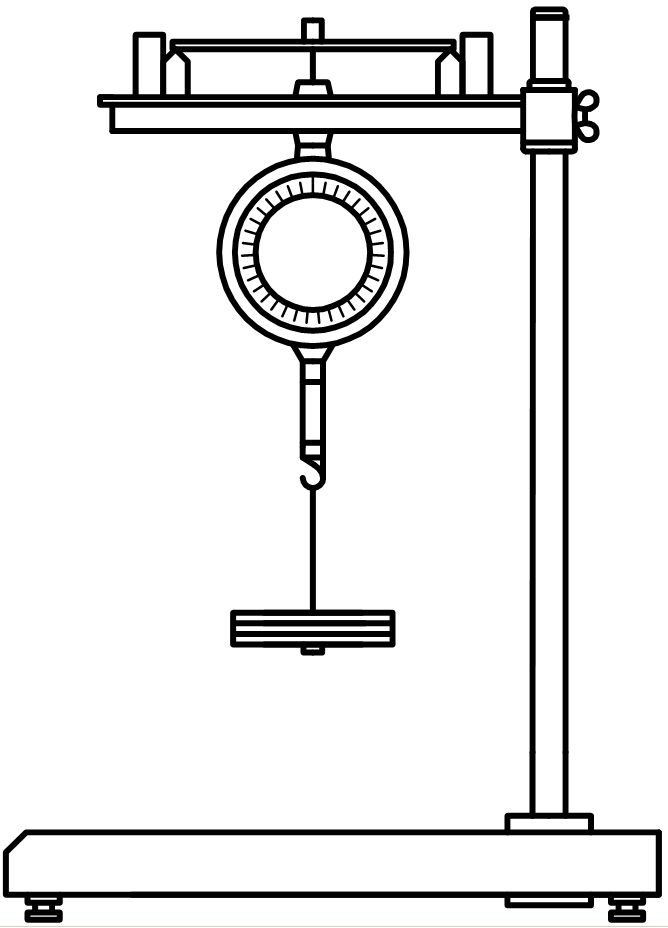
\includegraphics[width=0.35\linewidth, keepaspectratio=true]{M9-PlateBenderMachine}
\end{center}
\caption{\label{fig:m9b-equipment}}
\end{figure}

\begin{enumerate}
\item Установить одну из исследуемых пластин на призматические опоры и отрегулировать циферблатный индикатор таким образом, чтобы его острие касалось пластины.
\item Последовательно подвешивать на нагрузочную скобу индикатора гири различной массы, фиксируя по его шкале величину прогиба. Для повышения точности проводить измерения прогиба с гирей одного достоинства не менее пяти раз. Результаты заносить в таблицу протокола.
\item С помощью штангенциркуля определить линейные размеры исследуемой пластины. 
\item Вычислить модуль Юнга по расчетной формуле для каждого измерения и провести статистическую обработку результатов. \\
Расчетная формула: %может сделать ей номер...
\[
E = \frac{PL^3}{4bh^3x}, %ИЗМ: не вижу причин не делать тут \frac
\]
где $P$ "--- вес гири, $L$ "--- длина пластины, $h$ "--- ее толщина,  $b$ "--- ширина, $x$ "--- величина прогиба. \\
Все результаты измерений занесите в таблицу~\ref{tab:m9b-res-exp}. %мб вне enumerate

\begin{table}[h]
\caption{\label{tab:m9b-res-exp}}
\begin{center}
\begin{tabular}{|c|c|c|c|}
\hline %не ставлю номер, так каличество строк в таблице только указывает на то, что их должно быть много... тут вообще правильнее как с цилиндрами в intro делать, т. е. еще один столбец... ну да ладно... все равно эту работу никто не делает; правда, в связи с этим оставила 10 строк, потому что из работы следует, что число строк кратно пяти; я бы и до пяти сократила, а то не влезает, но нельзя
\multirow{2}*{\textnumero} & \multirow{2}{2.3cm}{\centering Масса груза,~кг} &  \multirow{2}{3.5cm}{\centering Растягивающая сила,~\Units{Н}} & \multirow{2}{3.5cm}{\centering Величина деформации,~\Units{м}} \\ %мб масса не груза, а гири; величина прогиба, а не деформации
& & & \\ \hline
& & & \\ \hline
& & & \\ \hline
& & & \\ \hline
& & & \\ \hline
& & & \\ \hline
& & & \\ \hline
& & & \\ \hline
& & & \\ \hline
& & & \\ \hline
& & & \\ \hline
\end{tabular}
\end{center}
\end{table}

\end{enumerate}

\subsection{Обработка результатов измерений}
По данным таблицы рассчитать средние значения измеренных величин и их средние квадратичные погрешности. 

Подставить полученные величины в формулу для вычисления относительной погрешности косвенных измерений: 
\[ %тот же вопрос: мб номер
\frac{\Delta E}{E} = \frac{\Delta P}{P} + 3\frac{\Delta L}{L} + \frac{\Delta b}{b} + 3\frac{\Delta h}{h} + \frac{\Delta x}{x}.
\]

\subsection{Контрольные вопросы}
\begin{enumerate}
\item Как связаны коэффициент жесткости и модуль Юнга?
\item Как изменяется жесткость пружины при изменении ее длины?
\item Найти жесткость системы из двух  пружин, соединенных последовательно (параллельно), если известны коэффициенты жесткости обеих: $k_1$ и $k_2$.
\item Изменится ли механическое напряжение образца, если вместо растяжения сжать его на ту же величину?
\item Во сколько раз необходимо увеличить силу, чтобы свитой шнур из четырех одинаковых проволочек получил такое же относительное удлинение, как и одна из них?
\item Во сколько раз увеличивается нагрузка на ноги собаки, когда ее рост увеличивается в два раза? Во столько же раз  изменяются и другие ее размеры.
\item Деформация протяженного тела возникает тогда, когда различные его части при поступательном движении совершают различные перемещения. Как сила упругости в некотором сечении тела зависит от положения этого сечения относительно точки приложения внешней силы?
\item С помощью закона Гука найдите удлинение подвешенного вертикально за один конец стержня под действием силы тяжести. Пусть известна первоначальная длина стержня, его плотность и модуль Юнга.
\end{enumerate}

\end{document}
